\documentclass{ximera}
\graphicspath{  %% When looking for images,
{./}            %% look here first,
{./pictures/}   %% then look for a pictures folder,
{../pictures/}  %% which may be a directory up.
{../../pictures/}  %% which may be a directory up.
{../../../pictures/}  %% which may be a directory up.
{../../../../pictures/}  %% which may be a directory up.
}

\usepackage{listings}
%\usepackage{circuitikz}
\usepackage{xcolor}
\usepackage{amsmath,amsthm}
\usepackage{subcaption}
\usepackage{graphicx}
\usepackage{tikz}
%\usepackage{tikz-3dplot}
\usepackage{amsfonts}
%\usepackage{mdframed} % For framing content
%\usepackage{tikz-cd}

  \renewcommand{\vector}[1]{\left\langle #1\right\rangle}
  \newcommand{\arrowvec}[1]{{\overset{\rightharpoonup}{#1}}}
  \newcommand{\ro}{\texttt{R}}%% row operation
  \newcommand{\dotp}{\bullet}%% dot product
  \renewcommand{\l}{\ell}
  \let\defaultAnswerFormat\answerFormatBoxed
  \usetikzlibrary{calc,bending}
  \tikzset{>=stealth}
  




%make a maroon color
\definecolor{maroon}{RGB}{128,0,0}
%make a dark blue color
\definecolor{darkblue}{RGB}{0,0,139}
%define the color fourier0 to be the maroon color
\definecolor{fourier0}{RGB}{128,0,0}
%define the color fourier1 to be the dark blue color
\definecolor{fourier1}{RGB}{0,0,139}
%define the color fourier 1t to be the light blue color
\definecolor{fourier1t}{RGB}{173,216,230}
%define the color fourier2 to be the dark green color
\definecolor{fourier2}{RGB}{0,100,0}
%define teh color fourier2t to be the light green color
\definecolor{fourier2t}{RGB}{144,238,144}
%define the color fourier3 to be the dark purple color
\definecolor{fourier3}{RGB}{128,0,128}
%define the color fourier3t to be the light purple color
\definecolor{fourier3t}{RGB}{221,160,221}
%define the color fourier0t to be the red color
\definecolor{fourier0t}{RGB}{255,0,0}
%define the color fourier4 to be the orange color
\definecolor{fourier4}{RGB}{255,165,0}
%define the color fourier4t to be the darker orange color
\definecolor{fourier4t}{RGB}{255,215,0}
%define the color fourier5 to be the yellow color
\definecolor{fourier5}{RGB}{255,255,0}
%define the color fourier5t to be the darker yellow color
\definecolor{fourier5t}{RGB}{255,255,100}
%define the color fourier6 to be the green color
\definecolor{fourier6}{RGB}{0,128,0}
%define the color fourier6t to be the darker green color
\definecolor{fourier6t}{RGB}{0,255,0}

%New commands for this doc for errors in copying
\newcommand{\eigenvar}{\lambda}
%\newcommand{\vect}[1]{\mathbf{#1}}
\renewcommand{\th}{^{\text{th}}}
\newcommand{\st}{^{\text{st}}}
\newcommand{\nd}{^{\text{nd}}}
\newcommand{\rd}{^{\text{rd}}}
\newcommand{\paren}[1]{\left(#1\right)}
\newcommand{\abs}[1]{\left|#1\right|}
\newcommand{\R}{\mathbb{R}}
\newcommand{\C}{\mathbb{C}}
\newcommand{\Hilb}{\mathbb{H}}
\newcommand{\qq}[1]{\text{#1}}
\newcommand{\Z}{\mathbb{Z}}
\newcommand{\N}{\mathbb{N}}
\newcommand{\q}[1]{\text{``#1''}}
%\newcommand{\mat}[1]{\begin{bmatrix}#1\end{bmatrix}}
\newcommand{\rref}{\text{reduced row echelon form}}
\newcommand{\ef}{\text{echelon form}}
\newcommand{\ohm}{\Omega}
\newcommand{\volt}{\text{V}}
\newcommand{\amp}{\text{A}}
\newcommand{\Seq}{\textbf{Seq}}
\newcommand{\Poly}{\textbf{P}}
\renewcommand{\quad}{\text{    }}
\newcommand{\roweq}{\simeq}
\newcommand{\rowop}{\simeq}
\newcommand{\rowswap}{\leftrightarrow}
\newcommand{\Mat}{\textbf{M}}
\newcommand{\Func}{\textbf{Func}}
\newcommand{\Hw}{\textbf{Hamming weight}}
\newcommand{\Hd}{\textbf{Hamming distance}}
\newcommand{\rank}{\text{rank}}
\newcommand{\longvect}[1]{\overrightarrow{#1}}
% Define the circled command
\newcommand{\circled}[1]{%
  \tikz[baseline=(char.base)]{
    \node[shape=circle,draw,inner sep=2pt,red,fill=red!20,text=black] (char) {#1};}%
}

% Define custom command \strikeh that just puts red text on the 2nd argument
\newcommand{\strikeh}[2]{\textcolor{red}{#2}}

% Define custom command \strikev that just puts red text on the 2nd argument
\newcommand{\strikev}[2]{\textcolor{red}{#2}}

%more new commands for this doc for errors in copying
\newcommand{\SI}{\text{SI}}
\newcommand{\kg}{\text{kg}}
\newcommand{\m}{\text{m}}
\newcommand{\s}{\text{s}}
\newcommand{\norm}[1]{\left\|#1\right\|}
\newcommand{\col}{\text{col}}
\newcommand{\sspan}{\text{span}}
\newcommand{\proj}{\text{proj}}
\newcommand{\set}[1]{\left\{#1\right\}}
\newcommand{\degC}{^\circ\text{C}}
\newcommand{\centroid}[1]{\overline{#1}}
\newcommand{\dotprod}{\boldsymbol{\cdot}}
%\newcommand{\coord}[1]{\begin{bmatrix}#1\end{bmatrix}}
\newcommand{\iprod}[1]{\langle #1 \rangle}
\newcommand{\adjoint}{^{*}}
\newcommand{\conjugate}[1]{\overline{#1}}
\newcommand{\eigenvarA}{\lambda}
\newcommand{\eigenvarB}{\mu}
\newcommand{\orth}{\perp}
\newcommand{\bigbracket}[1]{\left[#1\right]}
\newcommand{\textiff}{\text{ if and only if }}
\newcommand{\adj}{\text{adj}}
\newcommand{\ijth}{\emph{ij}^\text{th}}
\newcommand{\minor}[2]{M_{#2}}
\newcommand{\cofactor}{\text{C}}
\newcommand{\shift}{\textbf{shift}}
\newcommand{\startmat}[1]{
  \left[\begin{array}{#1}
}
\newcommand{\stopmat}{\end{array}\right]}
%a command to give a name to explorations and hints and theorems
\newcommand{\name}[1]{\begin{centering}\textbf{#1}\end{centering}}
\newcommand{\vect}[1]{\vec{#1}}
\newcommand{\dfn}[1]{\textbf{#1}}
\newcommand{\transpose}{\mathsf{T}}
\newcommand{\mtlb}[2][black]{\texttt{\textcolor{#1}{#2}}}
\newcommand{\RR}{\mathbb{R}} % Real numbers
\newcommand{\id}{\text{id}}
\newcommand{\coord}[1]{\langle#1\rangle}
\newcommand{\RREF}{\text{RREF}}
\newcommand{\Null}{\text{Null}}
\newcommand{\Nullity}{\text{Nullity}}
\newcommand{\Rank}{\text{Rank}}
\newcommand{\Col}{\text{Col}}
\newcommand{\Ef}{\text{EF}}
\newcommand{\boxprod}[3]{\abs{(#1\times#2)\cdot#3}}

\author{Zack Reed} %PEter Selinger
\title{Bringing Everything Together: Gauss and Echelon Forms}
\begin{document}
\begin{abstract}

\end{abstract}
\maketitle
    
\section*{Systems, Augmented Matrices and Elementary Row Operations}
 
\subsection*{Augmented Matrices}
 
We've been focusing on a few solution-preserving operations that can be carried out on systems of equations, called \emph{row operations}:
\begin{itemize}
\item Switching the order of equations $i$ and $j$: $R_i\leftrightarrow R_j$
\item Multiplying both sides of an equation by the same non-zero constant $\lambda$, $R_i\rightarrow\lambda R_i$
\item Adding a multiple of one equation to another, $R_i\rightarrow R_i+\lambda R_j$
\end{itemize}
 
 
When \href{https://ximera.osu.edu/appliedlinearalgebra/c3ChapterThree/learningActivities/m3LearningActivities/modThreeSystems/matricesAreSystemsOfEquations2}{balancing chemical equations} we tied these row operations to special, reversible matrices called \emph{elementary matrices}:

\begin{itemize}

  \item The \textbf{row swapping matrix} $E_{ij}$, the identity matrix with rows $i$ and $j$ swapped.
  
  $E_{12}$ performed on a $3\times 3$ matrix would be the matrix

  \begin{equation*}
    \begin{bmatrix}
      0 & 1 & 0 \\
      1 & 0 & 0 \\
      0 & 0 & 1
    \end{bmatrix}
  \end{equation*}

  \item The \textbf{scaling matrix} $E_{i}(\lambda)$ is the matrix that results from multiplying row $i$ of the identity matrix by the scalar $c$.
  
  $E_{2}(3)$ performed on a $3\times 3$ matrix would be the matrix

  \begin{equation*}
    \begin{bmatrix}
      1 & 0 & 0 \\
      0 & 3 & 0 \\
      0 & 0 & 1
    \end{bmatrix}.
  \end{equation*}

  \item The \textbf{row addition matrix} $E_{ij}(\lambda)$ is the matrix that results from adding $c$ times row $i$ to row $j$ of the identity matrix.
  
  $E_{3,2}(2)$ performed on a $3\times 3$ matrix would be the matrix

  \begin{equation*}
    \begin{bmatrix}
      1 & 0 & 0 \\
      0 & 1 & 0 \\
      0 & 2 & 1
    \end{bmatrix}.
  \end{equation*}

  This will add $2$ times the second row to the third row.

\end{itemize}
 
In this section, we explicitly draw connections between these two representations of the same operations, and seek an efficient method for simplifying a system so that a solution (if it exists) is determinable.
 
\begin{example}
Consider the linear system
\begin{equation}
  \begin{array}{ccccccccc}
      x &- &y&&&&&= &0 \\
     2x& -&2y&+&z&+&2w&=&4\\
     & &y&&&+&w&=&0\\
     & &&&2z&+&w&=&5
  \end{array}
\end{equation}

Our goal is to use elementary row operations to transform this system into an equivalent and solvable system of the form

\begin{equation}\begin{array}{ccccccccc}
      x & &&&&&&= &a \\
     & &y&&&&&=&b\\
     & &&&z&&&=&c\\
     & &&&&&w&=&d
    \end{array}
    \end{equation}  
  
We'll first perform these steps as we have been, using row operations, and then perform the same operations with elementary matrices, on what's called an \emph{augmented matrix} representation of the system.

We start by subtracting twice row 1 from row 2. ($R_2\rightarrow R_2-2R_1$)
 
$$\begin{matrix}
      x &- &y&+&0z&+&0w&= &0 \\
     0x& +&0y&+& 1z&+& 2w&=& 4\\
     0x& +&y&+&0z&+&w&=&0\\
     0x&+&0y&+&2z&+&w&=&5
    \end{matrix}$$

Next, we add row 3 to row 1. ($R_1\rightarrow R_1+R_3$) 

\begin{prompt}
 $$\begin{matrix}
      x &+ & \answer{0}y&+&\answer{0}z&+& \answer{1}w&= & \answer{0} \\
     0x& +&0y&+&z&+&2w&=&4\\
     0x& +&y&+&0z&+&w&=&0\\
     0x&+&0y&+&2z&+&w&=&5
    \end{matrix}$$
\end{prompt}


\begin{prompt} Subtract twice row 2 from row 4. ($R_4\rightarrow R_4-2R_2$)
$$\begin{matrix}
      x &+ &0y&+&0z&+&1w&= &0 \\
     0x& +&0y&+&z&+&2w&=&4\\
     0x& +&y&+&0z&+&w&=&0\\
     \answer{0}x&+&\answer{0}y&+& \answer{0}z&+& \answer{-3}w&=& \answer{-3}
    \end{matrix}$$
\end{prompt}

\begin{prompt} Divide row 4 by $-3$. ($R_4\rightarrow -\frac{1}{3}R_4$)
$$\begin{matrix}
      x &+ &0y&+&0z&+&1w&= &0 \\
     0x& +&0y&+&z&+&2w&=&4\\
     0x& +&y&+&0z&+&w&=&0\\
     \answer{0}x&+&\answer{0}y&+&\answer{0}z&+& \answer{1}w&=&\answer{1}
    \end{matrix}$$
\end{prompt}   

\begin{prompt} We will do three operations in one step.
$$R_1\rightarrow R_1-R_4$$
$$R_2\rightarrow R_2-2R_4$$
$$R_3\rightarrow R_3-R_4$$
$$\begin{matrix}
      x &+ &\answer{0}y&+&\answer{0}z&+& \answer{0}w&= & \answer{-1} \\
     \answer{0}x& +&\answer{0}y&+&\answer{1}z&+& \answer{0}w&=& \answer{2}\\
     \answer{0}x& +&\answer{1}y&+&\answer{0}z&+& \answer{0}w&=& \answer{-1}\\
     0x&+&0y&+&0z&+&1w&=&1
    \end{matrix}$$
\end{prompt}   

We now exchange rows 2 and 3. ($R_2\leftrightarrow R_3$)
\begin{equation}\label{eq:sys20rref1}
\begin{array}{ccccccccc}
      x &+ &0y&+&0z&+&0w&= &-1 \\
   0x& +&y&+&0z&+&0w&=&-1\\
   0x& +&0y&+&z&+&0w&=&2\\
     0x&+&0y&+&0z&+&w&=&1
    \end{array}
    \end{equation}
    If we drop all of the zero terms, we have:
    \begin{equation}\label{eq:sys20rrefnozeros}
    \begin{array}{ccccccccc}
      x & &&&&&&= &-1 \\
   & &y&&&&&=&-1\\
   & &&&z&&&=&2\\
     &&&&&&w&=&1
    \end{array}
    \end{equation}
Now we see that $(-1, -1, 2, 1)$ is the solution.
\end{example}
 
If we were to state this as matrix equations, this would be the matrix-vector Multiplications

$$M\vec{x}=\vec{b}$$

where $M_1$ is the matrix 

\begin{equation}
  M_1=\begin{bmatrix}
    1 & -1 & 0 & 0 \\
    2 & -2 & 1 & 2 \\
    0 & 1  & 0 & 1 \\
    0 & 0  & 2 & 1 \\
  \end{bmatrix}
\end{equation},

$\vec{x}$ is the vector

\begin{equation}
  \vec{x}=\begin{bmatrix}
    -1 \\
    -1  \\
    2 \\
    1  
  \end{bmatrix}
\end{equation},

and $\vec{b}$ is the vector

\begin{equation}
  \vec{b}=\begin{bmatrix}
    0 \\
    4  \\
    0 \\
    5  
  \end{bmatrix}
\end{equation}.

That's a key interpretation of the variables $x, y, z, w$ satisfying the system, is that the matrix-vector multiplication gives the vector represented by the right side of the equations.

\begin{remark}{MATLAB Check!}

  Let's check it in MATLAB! We can set up the matrix 

  \begin{verbatim}
  M=[1, -1, 0, 0;
      2, -2, 1, 2;
      0, 0, 2, 1]
  \end{verbatim}

  Then, we set up the potential solution vector 

  \begin{verbatim}
  x=[-1; -1; 2; 1]
  \end{verbatim}

  Then, we multiply $M*x$ and hope that it's $\vec{b}$!

  \begin{verbatim}
  b=M*x
  \end{verbatim}

  Thankfully, we get the right solution vector!

\end{remark}

This matrix-interpretation of the solution will become much more important in the next chapter, but for now we're going to use it to give us some slight notational convenience. 

\begin{remark}{Augmented Matrices}

If we change the system slightly, we can state the entire system as one matrix on which we can use elementary matrices to efficiently streamline this process, and to conveniently use MATLAB commands to our advantage.

Consider the system 

\begin{equation}
  \begin{array}{cccccccccc}
      x &- &y&&&&&-0&= &0 \\
     2x& -&2y&+&z&+&2w&-4&=&0\\
     & &y&&&+&w&-0&=&0\\
     & &&&2z&+&w&-5&=&0
  \end{array}
\end{equation}, 

which is our original system just after subtracting the constant terms from the right side to the left.

We can now represent this equivalent system with the same matrix as before, but now with the constant terms as well. We'll call this new matrix the \emph{augmented matrix} of the system, where the "augmentation" is just putting the constants on the left side.

\begin{equation}
  M_a=\begin{bmatrix}
    1 & -1 & 0 & 0 & 0\\
    2 & -2 & 1 & 2 & 4\\
    0 & 1  & 0 & 1 & 0\\
    0 & 0  & 2 & 1 & 5\\
  \end{bmatrix}
\end{equation}.

You'll notice that the constant terms aren't negative anymore. That's because we get to the system by the matrix vector multiplciation 

$M_a\vec{x}$, where 

\begin{equation}
  \vec{x}=\begin{bmatrix}
    x \\
    y  \\
    z \\
    w \\
    -1  
  \end{bmatrix}
\end{equation}.

The final coordinate of $-1$ in $\vec{x}$ is how we get the negative constant terms in our equivalent solution.

This is nice, because we can represent the \emph{entire} system of equations with \emph{just one} matrix, rather than having to coordinate lots of variables and constants and matrix-vector products.

Many use a vertical bar $|$ to represent that the final column contains constants, and we will adopt this practice as well. 

So we'd use the augmented matrix

\begin{equation}
  M_a=\left[\begin{array}{cccc|c}
    1 & -1 & 0 & 0 & 0\\
    2 & -2 & 1 & 2 & 4\\
    0 & 1  & 0 & 1 & 0\\
    0 & 0  & 2 & 1 & 5\\
  \end{array}\right]
\end{equation}

Now, rather than having to rewrite the system each time along with each row operations, we can keep track of the whole process just by using matrices and multiplication by elementary matrices!

\end{remark}

Let's re-do these steps, but at each stage track the augmented matrix after multiplying by elementary matrices:

Here's our starting matrix.

$$\left[\begin{array}{cccc|c} 
 1&-1&0&0&0\\2&-2&1&2&4\\0&1&0&1&0\\0&0&2&1&5
 \end{array}\right]$$

On the left side you'll see the elementary matrix being multiplied, and on the right you'll see the resulting augmented matrix.
 
$$\left[\begin{array}{cccc|c} 
 1&-1&0&0&0\\2&-2&1&2&4\\0&1&0&1&0\\0&0&2&1&5
 \end{array}\right]$$

 $$E_{12}(-2)\rightarrow%{R_2-2R_1}\\
 \left[\begin{array}{cccc|c} 
 1&-1&0&0&0\\0&0&1&2&4\\0&1&0&1&0\\0&0&2&1&5
 \end{array}\right]$$

 $$E_{3,1}(1)\rightarrow%{R_1+R_3}\\
\left[\begin{array}{cccc|c} 
 1&0&0&1&0\\2&-2&1&2&4\\0&1&0&1&0\\0&0&2&1&5
 \end{array}\right]$$

$$E_{2,4}(-2)\rightarrow%{R_4-2R_2}\\
\left[\begin{array}{cccc|c} 
 1&0&0&1&0\\0&0&1&2&4\\0&1&0&1&0\\0&0&0&-3&-3
 \end{array}\right]$$

$$E_4(-1/3)\rightarrow%{(-1/3)R_4}\\
 \left[\begin{array}{cccc|c} 
 1&0&0&1&0\\0&0&1&2&4\\0&1&0&1&0\\0&0&0&1&1
 \end{array}\right]$$

$$E_{4,1}(-1)\rightarrow%{R_1-R_4}\\
E_{4,2}(-2)\rightarrow%{R_2-2R_4}\\
E_{4,3}(-1)\rightarrow%{R_3-R_4}\\
\left[\begin{array}{cccc|c} 
 1&0&0&0&-1\\0&0&1&0&2\\0&1&0&0&-1\\0&0&0&1&1
 \end{array}\right]$$

 $$E_{23}\rightarrow%{R_2\leftrightarrow R_3}\\
 \left[\begin{array}{cccc|c}
  1&0&0&0&-1\\
  0&1&0&0&-1\\
  0&0&1&0&2\\
  0&0&0&1&1
\end{array}\right]$$ 


  
The last augmented matrix corresponds to the solution system, so again we've found the solution, but arguably in a slightly easier representation.

This utility compounds when we try to use technology to speed things up! In MATLAB, we can define functions to very quickly carry out these calculations, and ultimately we can have MATLAB do the entire process for us with one command, \texttt{rref}.

 

\begin{remark}\name{Formal Definitions}

  Let's formalize our definitions.  Every linear system
$$\begin{array}{ccccccccc}
      a_{11}x_1 &+ &a_{12}x_2&+&\ldots&+&a_{1n}x_n&= &b_1 \\
     a_{21}x_1 &+ &a_{22}x_2&+&\ldots&+&a_{2n}x_n&= &b_2 \\
     &&&&\vdots&&&& \\
     a_{m1}x_1 &+ &a_{m2}x_2&+&\ldots&+&a_{mn}x_n&= &b_m
    \end{array}$$
    can be written in the \dfn{augmented matrix form} as follows:
    $$\left[\begin{array}{cccc|c} 
 a_{11}&a_{12}&\ldots&a_{1n}&b_1\\a_{21}&a_{22}&\ldots&a_{2n}&b_2\\\vdots&\vdots&\ddots&\vdots&\vdots\\a_{m1}&a_{m2}&\ldots&a_{mn}&b_m
 \end{array}\right]$$
 The array to the left of the vertical bar is called the \dfn{coefficient matrix} of the linear system and is often given a capital letter name, like $A$.  The vertical array to the right of the bar is called a \dfn{constant vector}.
 $$A=\begin{bmatrix}a_{11}&a_{12}&\ldots&a_{1n}\\a_{21}&a_{22}&\ldots&a_{2n}\\\vdots&\vdots&\ddots&\vdots\\a_{m1}&a_{m2}&\ldots&a_{mn}\end{bmatrix}\quad\text{and}\quad\vec{b}=\begin{bmatrix}b_1\\b_2\\\vdots\\b_m\end{bmatrix}$$
We will sometimes use the following notation to represent an augmented matrix.
 
$$\left[\begin{array}{c|c} 
 A & \vec{b}\\
 \end{array}\right]$$

The same elementary row operations that we perform on a system of equations can be performed on the corresponding augmented matrix, or any matrix for that matter.  If a matrix can be obtained from another matrix by means of elementary row operations, we say that the two matrices are \dfn{row-equivalent}. 
\end{remark}




\begin{example}\label{init:backsub}
Let's try out augmented matrices in a new system, with the help of MATLAB!

First, consider the new system:



$$\begin{array}{ccccccc}
      x_1 &- &x_2&-&3x_3&= &1 \\
   4x_1& -&2x_2&-&7x_3&=&1\\
   -x_1& +&x_2&+&4x_3&=&1
    \end{array}$$

The corresponding augmented matrix is: 


 
\[\left[\begin{array}{ccc|c} 
 1&-1&-3&1\\4&-2&-7&1\\-1&1&4&1
 \end{array}\right]\]

 

 We then add $-4$ times row 1 to row 2, and then add row 1 to row 3. 

\end{example}


 
 \begin{remark}\name{MATLAB Help with Elementary Matrices}

 Rather than needing to rewrite the matrices each time, the course linalg folder has provided simple functions to make these elementary matrices.

The functions are \texttt{row\_add}, \texttt{row\_scale}, and \texttt{row\_swap}, which match the names of the elementary matrices. The arguments to these functions are always: 1st - the row(s) in the $ij$ order of the elementary matrices $E_{ij}$, 2nd - any scalars as necessary, 3rd - the dimension of the matrix. 


Adding $-4$ times row 1 to row 2 is 
$E_{12}(-4)=\begin{bmatrix}
1&0&0\\
-4&1&0\\
0&0&1
\end{bmatrix}$

The MATLAB function that will quickly give you this matrix is 

\begin{verbatim}
linalg.row_add(1,2,-4,3)
\end{verbatim}

Notice that the order of the entries in \texttt{row\_add} are the same as you would write in the elementary matrix, just with the added need to put a dimension down as well.

Then to add row 1 to row 3, you would input


\begin{verbatim}
linalg.row_add(1,3,1,3)
\end{verbatim}

You would then multiply them together, and then by $M$, to make the new augmented matrix. For instance:

\begin{verbatim}
M=[1, -1, -3, 1;
4, -2, -7, 1;
-1, 1, 4, 1]

aug=linalg.row_add(1,3,1,3)*linalg.row_add(1,2,-4,3)*M
\end{verbatim}

Which gives the same augmented matrix as you find below.

\end{remark}



 This yields

 $$
E_{1,2}(-4)\rightarrow%{R_2-4R_1}\\
E_{1,3}(1)\rightarrow%{R_3+R_1}\\
\left[\begin{array}{ccc|c} 
  1&\answer{-1}&-3&1\\\answer{0}&2&5&\answer{-3}\\0&0&1&2
  \end{array}\right]
$$

Now do the same (or go by hand) to carry out and verify the remaining row operations.

$$
E_{2}(1/2)\rightarrow
\left[\begin{array}{ccc|c} 
  1&-1&-3&1\\0&1&\answer{5/2}&\answer{-3/2}\\0&0&1&2
  \end{array}\right]
$$

$$$$
E_{2,1}(1)\rightarrow
\left[\begin{array}{ccc|c} 
  1&0&\answer{-1/2}&\answer{-1/2}\\0&1&5/2&-3/2\\0&0&1&2
  \end{array}\right]
$$



$$E_{3,1}(1/2)\rightarrow E_{3,2}(-5/2)\rightarrow
\left[\begin{array}{ccc|c} 
  1&0&0&1/2\\0&1&0&-13/2\\0&0&1&2
  \end{array}\right]$$


 
\begin{remark}

  You'll note that in each example, even when solving systems of equations, we've always ended with something as close to the identity matrix (on the left side of the augment) as possible. This is very intentional, and is called \emph{reduced row echelon form}.

  In essence, the reduced row echelon form (\texttt{rref}) gets us as close to back-substitution in the system of equations as possible. 

  This will become more formalized later, but for now note that there's actually a command in MATLAB that we can use to our advantage. 

  If we started with our same $M$, and did the following:

  \begin{verbatim}
M=[1, -1, -3, 1;
  4, -2, -7, 1;
  -1, 1, 4, 1]

M=sym(M)

aug=rref(M)
  \end{verbatim}

  We would have arrived at the same final result, immediately. NOTE: I use sym(M) because it keeps fractions and other variables at play, which can help the MATLAB output better align with the mathematics, rather than dealing with compounding decimal errors. 
  
  Essentially, MATLAB is doing the steps for us, in a process called \emph{Gaussian Eliminiation}, or more specifically for matrices \emph{Gauss-Jordan Elimination}

\end{remark}




This gives us the solution $(\frac{1}{2}, -\frac{13}{2}, 2)$.

Next, we'll put some formal definitions for the techniques we used here.
 

 
\subsection*{Row-Echelon and Reduced Row-Echelon Forms}

These definitions are here more for reference if needed, and it might help clear up some technicalities if you have trouble keeping the mechanics and interpretations of row operations and echelon forms straight. 

You won't necessarily be tested on this terminology, but again it might help to know this for your own use. In general, if you think about reduced row echelon form as "as close to the identity matrix above the diagonal as possible", you'll get the main idea.


 
\begin{definition}\label{def:leadentry} The first non-zero entry in a row of a matrix (when read from left to right) is called the \dfn{leading entry}.  When the leading entry is 1, we refer to it as a \dfn{leading 1}.
\end{definition}


 
\begin{definition}[Row-Echelon Form]\label{def:ref}
A matrix is said to be in \dfn{row-echelon form} if:
\begin{enumerate}
\item All entries below each leading entry are 0.
\item Each leading entry is in a column to the right of the leading entries in the rows above it.
\item All rows of zeros, if there are any, are located below non-zero rows.
\end{enumerate}
\end{definition}
 
The term row-echelon form can be applied to matrices whether or not they are augmented matrices (matrices with the vertical bar). For example, both the coefficient matrix and the augmented matrix in (\ref{eq:sys20rowechelon}) are in row-echelon form.  Note that the leading entries form a staircase pattern. All entries below the leading entries are zero, but the entries above the leading entries are not all zero.
 
Below are two more examples of matrices in row-echelon form.  The leading entries of each matrix are boxed.
$$\begin{bmatrix}
 \fbox{1}&2&-1&-5&0&2\\0&0&\fbox{3}&1&2&0\\0&0&0&0&\fbox{1}&0
 \end{bmatrix}\quad\text{and}\quad\begin{bmatrix}
 \fbox{4}&2\\0&\fbox{1}\\0&0
 \end{bmatrix}$$
  

The difference between the coefficient matrix in  (\ref{eq:sys20rowechelon}) and the coefficient matrix in (\ref{eq:sys20reducedrowechelon}) is that the leading entries of the  matrix in (\ref{eq:sys20reducedrowechelon}) are all 1's, and the matrix has zeros above each leading 1.  This motivates our next definition.
 
\begin{definition}[Reduced Row-Echelon Form]\label{def:rref}
A matrix that is already in \dfn{row-echelon} form is said to be in \dfn{reduced row-echelon form} if:
\begin{enumerate}
\item Each leading entry is $1$
\item All entries {\it above} and below each leading $1$ are $0$
\end{enumerate}
\end{definition}

The following two matrices are in \dfn{reduced row-echelon form}.  Note that there are $0$'
s below and above each leading $1$.
 
$$\begin{bmatrix} 
 \fbox{1}&0&-1&0&1\\0&\fbox{1}&0&0&2\\0&0&0&\fbox{1}&2
 \end{bmatrix}\quad\text{and}\quad\begin{bmatrix}
 \fbox{1}&0\\0&\fbox{1}\\0&0
 \end{bmatrix}$$
  
 When solving linear systems using the augmented matrix notation, our goal will be to transform the augmented matrix $M=[A|\vec{b}]$ into a row-echelon or reduced row-echelon form.  The reduced row-echelon form of $M$ is denoted by
$\mbox{rref}(M)$.  As we transform the augmented matrix $M$ to its reduced row-echelon form, the coefficient matrix $A$ (the matrix to the left of the bar) also gets transformed to its reduced row-echelon form, $\mbox{rref}(A)$.
 
 
\begin{example}\label{ex:freevar1} Solve the system of equations or determine that the system is inconsistent.
$$\begin{array}{ccccccccc}
      x &- &2y&+&z&&&= &2 \\
     -2x& +&y&-&z&+&w&=&0\\
     x& +&4y&&&+&w&=&1
    \end{array}$$



We want to start foregounding the interpretation of the \rref, so we'll start using the \texttt{rref} command to cut to the chase, and leave some row operations practice for the homework.

Use MATLAB to find the \rref of the augmented matrix associated with the system. 



$$\left[\begin{array}{cccc|c} 
 1&0&0&\answer{-5/3}&-3\\0&1&\answer{0}&\answer{2/3}&1\\0&0&\answer{1}&\answer{3}&7
 \end{array}\right]$$



 \begin{feedback}
 
  How'd it go? Don't forget to enter the system as a augmented matrix first. If you're having trouble, try

  \begin{verbatim}
  M=[1, -2, 1, 0, 2;
  -2, 1, -1, 1, 0;
  1, 4, 0, 1, 1]

  M=sym(M)

  rref(M)
  \end{verbatim}

 \end{feedback}
  
This \texttt{rref} matrix is not quite as nice as the our earlier matrices, and is more reminiscent of the balanced chemical equations that had many possible solutions. It is, however, in reduced row-echelon form.  

Let's see if (and how many) solutions exist for the system!

We have:
 $$\begin{array}{ccccccccc}
      x & &&&&-&(5/3)w&= &-3 \\
     & &y&&&+&(2/3)w&=&1\\
     & &&&z&+&3w&=&7
    \end{array}$$

If we re-write the system similar to our solutions in the chemical equation balancing, then we can explicitly write the row variables $x, y, $ and $z$ in terms of $w$ for suitably chosen $w$.

 $$\begin{array}{ccccccccc}
      x & &&&&&&= &-3+(5/3)w \\
     & &y&&&&&=&1-(2/3)w\\
     & &&&z&&&=&7-3w
    \end{array}$$

For example, let $w=0$, then $x=-3$, $y=1$ and $z=7$, so $(-3, 1, 7, 0)$ is a solution.  If we let $w=3$, then $x=2$, $y=-1$ and $z=-2$, so $(2, -1, -2, 3)$ is also a solution.

  We can think of the solution set in two different ways.  First, the solution set is the set of all points of the form$$\left(-3+\frac{5}{3}w, 1-\frac{2}{3}w, 7-3w, w\right)$$
  
If we want to think in terms of the hyperplane geometry of the system, then we could write 

 \begin{align*}
 x&=-3+\frac{5}{3}t\\
 y&=1-\frac{2}{3}t\\
 z&=7-3t\\
 w&=t.
 \end{align*}

 In this case, since $w$ is a dimension of the hyperplane, we let it vary and assign what's called a \emph{parameter}. These are called \emph{parametric equations} of the system. These will come up from time to time, so you'll want to be accustom to seeing and interpreting parametric equations.

To answer our original question, the system has infinitely many solutions, and is therefore consistent!
 
\end{example}
 
Observe that in Example \ref{ex:freevar1}, variables $x$, $y$ and $z$ correspond to the leading $1's$ in the reduced row-echelon.  We say that $x$, $y$ and $z$ are the \dfn{leading variables}.  Variable $w$ is not a leading variable; we refer to it as a \dfn{free variable} and assign a \dfn{parameter} $t$ to it.
 
\begin{example}\label{ex:nosolutionssys}
Solve the system of equations or determine that the system is inconsistent.
$$\begin{array}{ccccccc}
      2x & -&y&&&= &2 \\
     x& +&y&-&2z&=&0\\
     -3x& &&+&2z&=&-1
    \end{array}$$
     
    \begin{explanation}
    Rewrite the system in augmented matrix form, and use \texttt{rref} to put the augmented matrix into \rref.

    You'll get the following:
     
   \begin{equation}\label{eq:sys20nosolutionsys} \left[\begin{array}{ccc|c} 
 2&-1&0&2\\1&1&-2&0\\-3&0&2&-1
 \end{array}\right]\begin{array}{c}
 \\
 \rightsquigarrow\\
 \\
 \end{array}\left[\begin{array}{ccc|c} 
 1&0&\answer{-2/3}&\answer{0}\\0&1&\answer{-4/3}&\answer{0}\\0&0&\answer{0}&\answer{1}
 \end{array}\right]\end{equation}
     
 Converting back to a system of linear equations, we get
  
 \begin{equation}\label{eq:sys20nosolutions}\begin{array}{ccccccc}
      0x &+ &0y&-&\answer{(2/3)z}&= &\answer{0} \\
     0x&+ &0y&-&\answer{(4/3)z}&=&\answer{0}\\
     0x&+ &0y&+&\answer{0z}&=&\answer{1}
    \end{array}\end{equation}

    The last equation in this system clearly has no solutions.  We conclude that this system (and the original system) is inconsistent.

    \end{explanation}
     
\end{example}
 
\begin{observation}\label{ob:inconsistent} Note that the last row of the reduced row-echelon form in (\ref{eq:sys20nosolutionsys}) looks like this
$$\left[\begin{array}{ccc|c} 
 0&0&0&1
 \end{array}\right]$$

 This row corresponds to the equation

 $$\begin{array}{ccccccc}
     0x&+ &0y&+&0z&=&1
    \end{array}$$

 which clearly has no solutions. 
  
 In general, if the reduced row-echelon form of the augmented matrix contains a row

 $$\left[\begin{array}{ccc|c} 
 0&\ldots&0&1
 \end{array}\right]$$

 we can conclude that the system is inconsistent.
\end{observation}
 
\begin{example}\label{ex:rrefinfmanysolutionssys}
Solve the system of equations or determine that the system is inconsistent.
$$\begin{array}{ccccccc}
      x & -&3y&-&z&= &3 \\
     -3x& +&5y&&&=&-2\\
     x&+ &y&+&2z&=&-4
    \end{array}$$
     
    \begin{explanation}
    We rewrite the system in the augmented matrix form and transform it to reduced row-echelon form.  We leave the details of the elementary row operations to the reader and state the final result.
     
   $$ \left[\begin{array}{ccc|c} 
 1&-3&-1&3\\-3&5&0&-2\\1&1&2&-4
 \end{array}\right]\begin{array}{c}
 \\
 \rightsquigarrow\\
 \\
 \end{array}\left[\begin{array}{ccc|c} 
 1&0&5/4&-9/4\\0&1&3/4&-7/4\\0&0&0&0
 \end{array}\right]$$
 Converting the augmented matrix back to a system of equations we get
 $$\begin{array}{ccccccc}
      x &+ &0y&+&(5/4)z&= &-9/4 \\
     0x& +&y&+&(3/4)z&=&-7/4\\
     0x&+ &0y&+&0z&=&0
    \end{array}$$
     
 Unlike the last equation in (\ref{eq:sys20nosolutions}), the last equation in this system has infinitely many solutions because all values of $x$, $y$ and $z$ satisfy it.  Since the last equation contributes nothing, we will remove it and rewrite the system as
 $$\begin{array}{ccccc}
      x & &&= &-9/4-(5/4)z \\
     & &y&=&-7/4-(3/4)z\\
    \end{array}$$
Variables $x$ and $y$ correspond to leading $1's$ in the reduced row-echelon form.  So, $x$ and $y$ are the leading variables.    Variable $z$ is a free variable.  We let $z=t$.  Solutions to this system are points of the form
  $$\left(-\frac{9}{4}-\frac{5}{4}t, -\frac{7}{4}-\frac{3}{4}t, t\right)$$
  We can also interpret the solutions as lying on a line in $\RR^3$ given by parametric equations
  \begin{align*}
  x&=-\frac{9}{4}-\frac{5}{4}t\\
  y&=-\frac{7}{4}-\frac{3}{4}t\\
  z&=t\\
  \end{align*}
   
  This line is the line of intersection of the three planes.
 \end{explanation}
 \end{example}

\section*{Gaussian Elimination}
\subsection*{Row Echelon and Reduced Row Echelon Forms}
 
In general, there are many possible paths to reduced row echelon forms, however once the reduced row echelon form is reached, it's unique! This is summarized in the following diagram. (NOTE: We use the term "row echelon forms" when the leading entries are not 1. This creates many paths to an \rref)
 
\begin{center}
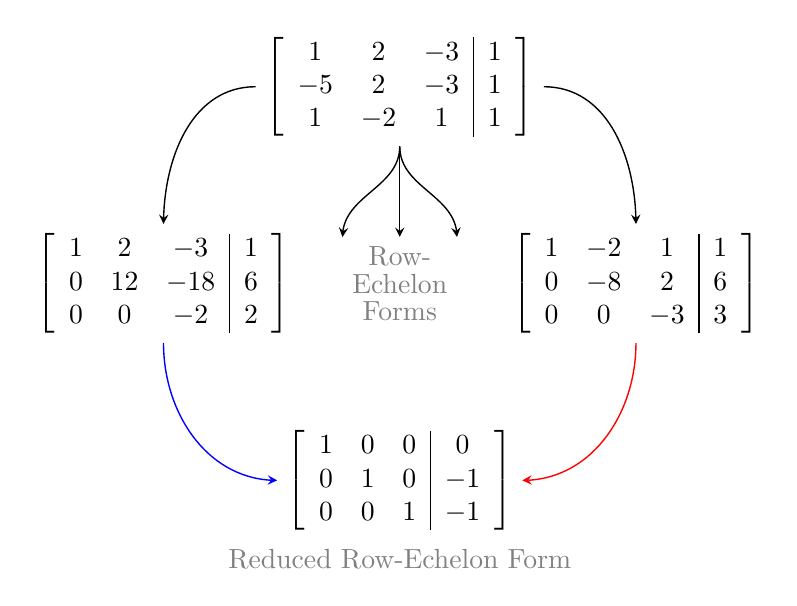
\begin{tikzpicture}
  \node[] at (0, 0)  (o)    {$\left[\begin{array}{ccc|c} 
 1&2&-3&1\\-5&2&-3&1\\1&-2&1&1
 \end{array}\right]$};
 \node[] at (-3, -2.5)  (left1)    {$\left[\begin{array}{ccc|c} 
 1&2&-3&1\\0&12&-18&6\\0&0&-2&2
 \end{array}\right]$};
 \node[] at (3, -2.5)  (right1)    {$\left[\begin{array}{ccc|c} 
 1&-2&1&1\\0&-8&2&6\\0&0&-3&3
 \end{array}\right]$};
 \node[gray] at (0, -2.5)  (c1)    {\shortstack{Row-\\Echelon\\Forms}};
 \node[] at (0, -5)  (c2)    {$\left[\begin{array}{ccc|c}  1&0&0&0\\0&1&0&-1\\0&0&1&-1
 \end{array}\right]$};
 \node[gray] at (0, -6)  (c3)    {Reduced Row-Echelon Form};
  
 \draw [->,line width=0.5pt,-stealth]  (o.west)to[out=180, in=90](left1.north);
  \draw [->,line width=0.5pt,-stealth]  (o.south)to[out=270, in=90](c1.north west);
  \draw [->,line width=0.5pt,-stealth]  (o.south)to[out=270, in=90](c1.north east);
  \draw [->,line width=0.5pt,-stealth]  (o.south)to[out=270, in=90](c1.north);
 \draw [->,line width=0.5pt,-stealth]  (o.east)to[out=0, in=90](right1.north);
 \draw [->,line width=0.5pt,-stealth,blue]  (left1.south)to[out=270, in=180](c2.west);
 \draw [->,line width=0.5pt,-stealth,red]  (right1.south)to[out=270, in=0](c2.east);
 \end{tikzpicture}
 \end{center}

 We tend to state useful mathematical facts as theorems. Here we state the uniqueness of the \rref.

 
\begin{theorem}\label{th:uniquenessofrref} The reduced row-echelon form of a matrix is unique.
\end{theorem}
A proof of this result can be found in [Yuster].
 
\section*{Gaussian and Gauss-Jordan Elimination}
 
\begin{definition}[Gaussian Elimination]\label{def:GaussianElimination}
The process of using the elementary row operations on a matrix to transform it into row-echelon form is called \dfn{Gaussian Elimination}.
\end{definition}
 
As we saw, it is possible to follow different sequences of row operations to arrive at various row-echelon forms.  However, it was not clear whether it is {\it always possible} to find a row-echelon form.  The following algorithm takes any matrix (or augmented matrix) and transforms it into row-echelon form:
\begin{algorithm}[Gaussian Algorithm] \label{alg:gaussian}
Let $A$ be an $m\times n$ matrix.

 
Set $i=1$ initially.
\begin{itemize}
\item[] Step 1. If $A$ consists entirely of zeros, stop;  $A$ is already in row-echelon form.
 
\item[] Step 2. Otherwise, find the first column from the left containing a nonzero entry in row $i$ or below row $i$.  This column will be called a \dfn{pivot column}.  Go down the pivot column, beginning with row $i$. Pick the topmost nonzero entry and call it $a$. If $a$ is not in row $i$, switch rows so that $a$ moves to row $i$.  Now $a$ is the \dfn{leading entry} in its row.  We will also refer to $a$ as a \dfn{pivot}. 
 
\item[] Step 3. By subtracting multiples of the row containing $a$ from rows below it, make each entry below $a$ zero.
 
\item[] Step 4.  Set $i=i+1$.  If $i > m$ then stop; $A$ is in row-echelon form.
 
\end{itemize}
 
Repeat steps 1--4 on the matrix consisting of the remaining rows.
When the process stops, $A$ will be in row echelon form.
\end{algorithm}

Gaussian Algorithm guarantees that every matrix will have a row-echelon form. 

\begin{definition}[Gauss-Jordan Elimination]\label{def:GaussJordanElimination}
  The process of using the elementary row operations on a matrix to transform it into \textbf{reduced} row-echelon form is called \dfn{Gauss-Jordan elimination}.
  \end{definition}

  \begin{algorithm}[Gauss-Jordan Algorithm] \label{alg:gauss-jordan}
    Let $A$ be an $m\times n$ matrix.
    Follow the steps of the Gaussian Algorithm but modify Step 2 to create leading $1's$ by multiplying the row containing $a$ by $\frac{1}{a}$.
    %Set $i=1$ initially.
    %\begin{itemize}
    %\item[] Step 1. If $A$ consists entirely of zeros, stop.  $A$ is already in row-echelon form.
     
    %\item[] Step 2*. Otherwise, find the first column from the left containing a nonzero entry in row $i$ or below row $i$.  This column will be called a \dfn{pivot column}.  Scan the pivot column from top to bottom, starting with row $i$.  Pick the topmost nonzero entry and call it $a$.  Switch rows, if necessary, to move the row containing $a$ to row $i$.  Now $a$ is the \dfn{leading entry} in its row.  We will also refer to $a$ as a \dfn{pivot}.  Multiply the row containing $a$ by $\frac{1}{a}$ to create a leading $1$. 
     
    %\item[] Step 3*. By subtracting multiples of the row containing the leading $1$ from rows {\it above} and below it, make each entry above and below the leading $1$ zero.
     
    %\item[] Step 4.  Set $i=i+1$.  If $i&gt;m$ then stop, and $A$ will be in row-echelon form.
     
    %\end{itemize}
     
    %Repeat steps 1--4 on the matrix consisting of the remaining rows.
    %When the process stops, $A$ will be in reduced row echelon form.
    When the Gaussian Algorithm terminates, subtract multiples of the rows containing leading $1's$ from the rows above to make all entries above the pivots zero.
    \end{algorithm}


 
\begin{example}\label{ex:non-augmented}
 
Use the Gaussian Algorithm to find a row-echelon form of $A$ if $$A=\begin{bmatrix}2&4\\1&2\\-1&1\\3&5\end{bmatrix}$$
\begin{explanation}
Following Step 2, we choose the first entry, $2$, as our pivot.  We then perform step 3, using the top row to get zeros in all entries below the $2$.
$$\begin{bmatrix} \fbox{$2$}&4\\1&2\\-1&1\\3&5\end{bmatrix}
  \begin{array}{c}
  \\
  \xrightarrow{R_2-(1/2)R_1}\\
  \xrightarrow{R_3+(1/2)R_1}\\
 \xrightarrow{R_4-(3/2)R_1}\\
 \end{array}
\begin{bmatrix}2&4\\0&0\\0&3\\0&-1\end{bmatrix}
$$
The first row is now complete, and we repeat the process on the rows below it. We identify $3$ as a pivot entry in the second column and move the row containing $3$ to be directly below the first completed row.  We then use the $3$ to make each entry below the $3$ a zero. 
 
$$\begin{bmatrix}2&4\\0&0\\0&\fbox{$3$}\\0&-1\end{bmatrix}
\xrightarrow{R_2\leftrightarrow R_3}\\
\begin{bmatrix}2&4\\0&\fbox{$3$}\\0&0\\0&-1\end{bmatrix}
  \begin{array}{c}
 \\
\\
  \\
 \xrightarrow{R_4+\frac{1}{3}R_2}\\
 \end{array}
 \begin{bmatrix}2&4\\0&3\\0&0\\0&0\end{bmatrix}
$$
This time the algorithm terminates since row 3 and row 4 are zero rows.
\end{explanation}
\end{example}
 
Given a matrix in row-echelon form, it is easy to bring it the reduced row-echelon form.  For example, continuing with Example \ref{ex:non-augmented}, we can start where we left off and compute $\mbox{rref}(A)$.  From our earlier computations we have:
 
$$\begin{bmatrix}2&4\\-1&1\\3&5\\1&2\end{bmatrix}\rightsquigarrow\begin{bmatrix}2&4\\0&3\\0&0\\0&0\end{bmatrix}$$
 
Now we create leading $1's$ and use them to to wipe out all non-zero entries above them.
$$\begin{bmatrix}2&4\\0&3\\0&0\\0&0\end{bmatrix}
  \begin{array}{c}
    \xrightarrow{(1/2)R_1}\\
  \xrightarrow{(1/3)R_2}\\
  \\
  \\
 \end{array}
\begin{bmatrix}1&2\\0&1\\0&0\\0&0\end{bmatrix}
  \begin{array}{c}
  \xrightarrow{R_1-2R_2}\\
\\
\\
 \\
 \end{array}
\begin{bmatrix}1&0\\0&1\\0&0\\0&0\end{bmatrix}=\mbox{rref}(A)$$
 
The following modification to the Gaussian Algorithm produces the reduced row-echelon form of a matrix.  This algorithm guarantees the existence of the reduced row-echelon form.

 
\begin{example}\label{ex:gaussjordanalg}
Use the Gauss-Jordan Algorithm to solve the system
$$\begin{array}{ccccccccc}
      3x &+ &y&+&7z&= &7 \\
     5x& +&3y&+&9z&=&13\\
      2x&+ &y&+&4z&=&5
    \end{array}$$
\begin{explanation}
\begin{align*}&\left[\begin{array}{ccc|c} 
 \fbox{$3$}&1&7&7\\5&3&9&13\\2&1&4&5
 \end{array}\right]\\
 \begin{array}{c}
  \xrightarrow{\frac{1}{3}R_1}\\
\\
\\
 \end{array}
 &\left[\begin{array}{ccc|c} 
 \fbox{$1$}&1/3&7/3&7/3\\5&3&9&13\\2&1&4&5
 \end{array}\right]\\
 \begin{array}{c}
 \\
 \xrightarrow{R_2-5R_1}\\
\\
\end{array}
&\left[\begin{array}{ccc|c} 
 \fbox{$1$}&1/3&7/3&7/3\\0&4/3&-8/3&4/3\\2&1&4&5
 \end{array}\right]\\
 \begin{array}{c}
  \\
\\
 \xrightarrow{R_3-2R_1}\\
\end{array}&\left[\begin{array}{ccc|c} 
 1&1/3&7/3&7/3\\0&\fbox{$4/3$}&-8/3&4/3\\0&1/3&-2/3&1/3
 \end{array}\right]\\
 \begin{array}{c}
\\
 \xrightarrow{\frac{3}{4}R_2}\\
\\
\end{array}
&\left[\begin{array}{ccc|c} 
 1&1/3&7/3&7/3\\0&\fbox{$1$}&-2&1\\0&1/3&-2/3&1/3
 \end{array}\right]\\
 \begin{array}{c}
\\
\\
 \xrightarrow{R_3-\frac{1}{3}R_2}\\
\end{array}
&\left[\begin{array}{ccc|c} 
 1&1/3&7/3&7/3\\0&\fbox{$1$}&-2&1\\0&0&0&0
 \end{array}\right]\\
 \begin{array}{c}
 \xrightarrow{R_1-\frac{1}{3}R_2}\\
 \\
\\
\end{array}
&\left[\begin{array}{ccc|c} 
 1&0&3&2\\0&1&-2&1\\0&0&0&0
 \end{array}\right]
 \end{align*}
  
 We convert the reduced row-echelon form to a system of equations and find the solution.  The last equation contributes nothing to the system so we omit writing it down.
  
 $$\begin{array}{ccccccccc}
      x & &&+&3z&= &2 \\
     & &y&-&2z&=&1
    \end{array}$$
    The solution is
    $$x=2-3t,\quad y=1+2t,\quad z=t$$
\end{explanation}
\end{example}

The Gauss-Jordan Algorithm guarantees the existence of the reduced row-echelon form for all matrices. In practice, we will be using \texttt{rref} to apply a similar algorithm in MATLAB, and our task will be interpreting the results!

\section*{Example Source}

This section is an adaptation of Anna Davis' Ximera text %FOUND HERE!

Davis' text was an adaptation pulling from the following open source texts:
 
Linear system in Exploration \ref{init:augmentedmatrixex} comes from Jim Hefferon's \href{http://joshua.smcvt.edu/linearalgebra/#current_version}{\it Linear Algebra}. (CC-BY-NC-SA)
 
Jim Hefferon, {\it Linear Algebra}, 3rd edition, page 6.

 Section 1.2 of Keith Nicholson's \href{https://open.umn.edu/opentextbooks/textbooks/linear-algebra-with-applications}{\it Linear Algebra with Applications}.
 
W. Keith Nicholson, {\it Linear Algebra with Applications}, Lyryx 2018, Open Edition, p 15-17.
 
\section*{Bibliography}
 
[Yuster] Thomas Yuster, The Reduced Row Echelon Form of a Matrix is Unique: a
Simple Proof, Mathematics Magazine, vol. 57, no. 2 (Mar. 1984), pp. 93-94.
 
\end{document}